% Created 2023-01-12 Thu 12:52
% Intended LaTeX compiler: pdflatex
\documentclass[11pt]{article}
\usepackage[utf8]{inputenc}
\usepackage[T1]{fontenc}
\usepackage{graphicx}
\usepackage{longtable}
\usepackage{wrapfig}
\usepackage{rotating}
\usepackage[normalem]{ulem}
\usepackage{amsmath}
\usepackage{amssymb}
\usepackage{capt-of}
\usepackage{hyperref}
\usepackage[polish]{babel}
\usepackage[margin=3cm]{geometry}
\author{nil}
\date{\today}
\title{}
\hypersetup{
 pdfauthor={nil},
 pdftitle={},
 pdfkeywords={},
 pdfsubject={},
 pdfcreator={Emacs 30.0.50 (Org mode 9.6)}, 
 pdflang={Polish}}
\begin{document}

\tableofcontents

\newpage
\section{Tranzystor bipolarny}
\label{sec:orga3c79a4}
\subsection{Poprawa 1}
\label{sec:orgd7401cd}
\begin{enumerate}
\item Układy pracy tranzystora bioplarnego. narysować i podpisać.
\label{sec:org7709c0c}
\item Charakterystki w układzie wspólnego emitera
\label{sec:org87b68d1}
\end{enumerate}
\subsection{Poprawa 2}
\label{sec:org1d156fc}
\begin{enumerate}
\item Charakterystki w układzie wspólnego emitera
\label{sec:orgb0bc1bb}
\item Zakresy pracy i warunki ich uzyskania.
\label{sec:org2bfbf43}
\begin{figure}[htbp]
\centering
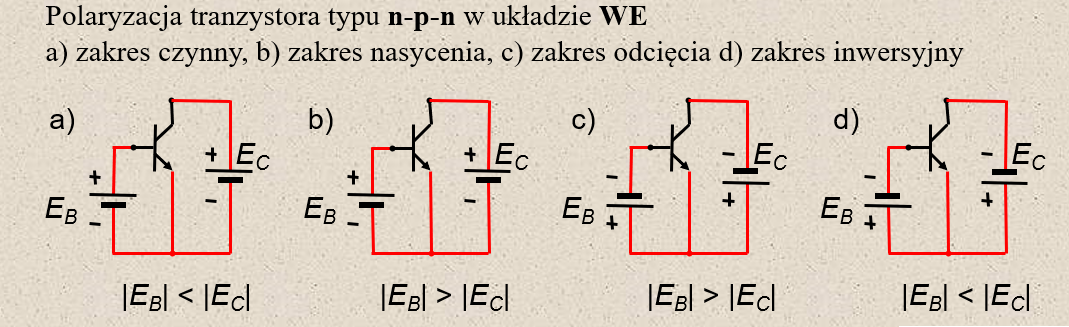
\includegraphics[width=.9\linewidth]{img/tranzystorBipolarny/zakresy.png}
\caption{Z prezentacji z moodla}
\end{figure}
\newpage
\end{enumerate}
\section{Tranzystor polowy}
\label{sec:org73b6eac}
\subsection{Poprawa 1}
\label{sec:orgb11557d}
\begin{enumerate}
\item charakterystki tranzystora polowego
\label{sec:orgafac88c}
\begin{figure}[htbp]
\centering
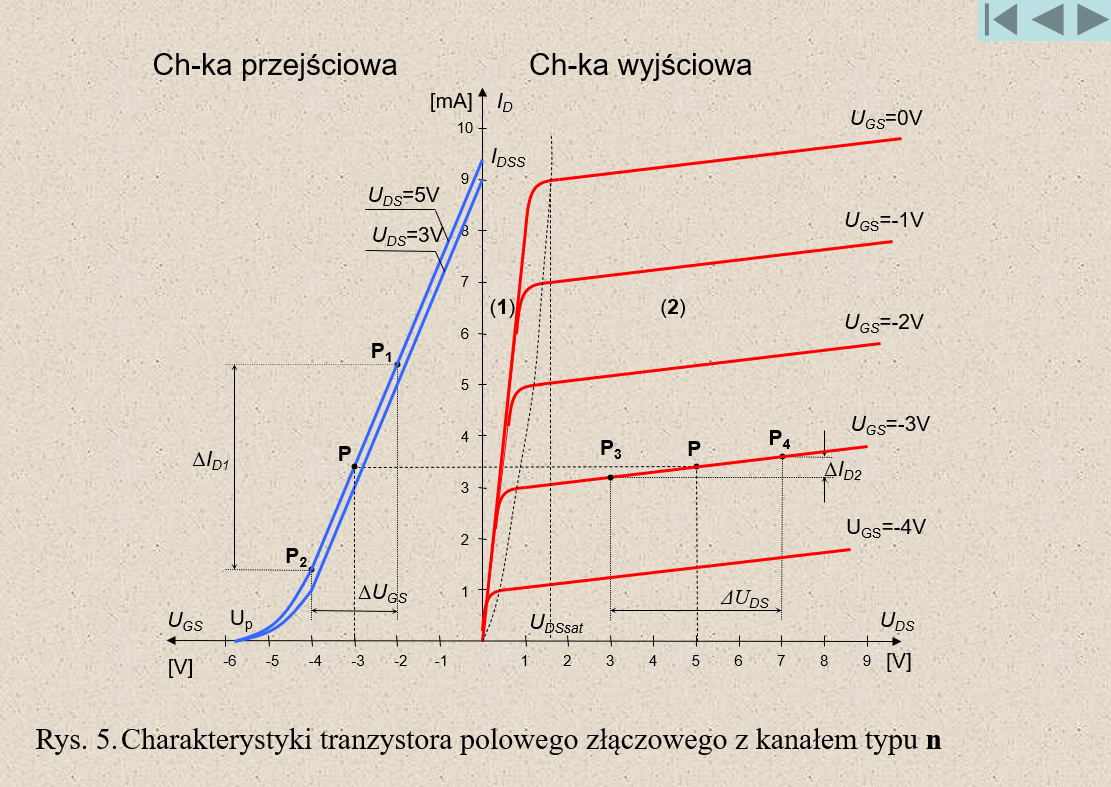
\includegraphics[width=.9\linewidth]{img/tranzystorPolowy/charakterystykaN.png}
\caption{Z prezentacji z moodla}
\end{figure}
\item transkonduktacnja wzór i wyznaczanie z charakterysyk
\label{sec:orgbdd04d8}
\end{enumerate}
\section{Zasilacze jakieśtam (5)}
\label{sec:orgf8910c4}
\end{document}